\documentclass[12pt]{article}
%\usepackage[a4paper,left=2cm,right=2cm,top=2cm,bottom=2cm]{geometry}
\usepackage{graphicx}
\usepackage[utf8]{inputenc}
\usepackage{float}
\usepackage{caption}
\usepackage{amsmath}
\usepackage[backend=biber]{biblatex}
\usepackage{amssymb}
\bibliography{literature.bib}
\title{Machine Learning: Final project bomberchamp}
\date{today}
\begin{document}





\section{Introduction}
% Introduction
% we implemented a rainbow dqn

\subsection{Reinforcement Learning}
% Reinforcement Learning basics a
\subsection{Neural Networks}
% basics j

\section{DQN}
% a

\section{Rainbow / DQN Extensions}
\subsection{Double DQN} % a
\subsection{Dueling DQN} % a
\subsection{Prioritized Replay Buffer} % a
\subsection{Noisy} % a
\subsection{Multi-Step Learning} % j
% 

\section{Other things}
\subsection{Augmented data}
\subsection{Centring of agent} % j / a
\subsection{Invalid actions} % 
\subsection{Auxilliary Reward Design}
\subsection{Minigame Collection} % j
\subsection{Self-Play (maybe)}

\section{Observation}
\subsection{It does not work}
% nothing works
% solution: make it better
\subsection{Network scaling} % j
% different networks from minigame to full game
% lots of graphs

% our learning process


\section{Summary and Improvements}
% improvements: distributional DQN, train for 3 months

% improvement of game setup: j
% - make provided framework easy to use
% -- currently main.py, settings.py and possibly callbacks.py has to be changed for a simple switch between train and test mode
% -- separate rendering and environment, so that the environment can be called from e.g. a jupyter notebook
% -- provide main.py or python notebook 





\section{Model}
In reinforcement learning, an agent needs to learn how to act optimally in sequential decision making problems by maximizing a reward signal. This means, that the agent is provided with some kind of input state and then needs to choose an action. The subsequent state, depends on the chosen action and the input state. This subsequent state as well as an reward based on how well the agent performed is given back to the agent. To find a good policy on how to act, the agent needs to optimize these rewards.
The true value of an action under a chosen policy is defined as the sum of the current reward for that action and the discounted future rewards:
\begin{equation}
Q_\pi(s,a)= E\left[\sum_{n=1}^{\infty} \gamma^{n-1}R_n^n\right] \Bigg|_{a,s,\pi}.
\end{equation} 
$\gamma\,\epsilon\,[0,1]$ denotes the discounting factor.
The best policy is then determined by maximizing $Q_\pi$ over the actions in every step.
\subsection{Q-learning}
Usually it is not possible to learn every action for every state explicitly because the problems are often to extensive. Therefore The Q-values get approximated by a parametrized function $Q(a,s,\theta_t)$. Which is updated towards the target value $Y_{t}^{\mathrm{Q}}$:
\begin{equation}
Y_{t}^{\mathrm{Q}} \equiv R_{t+1}+\gamma \max _{a} Q\left(S_{t+1}, a ; \boldsymbol{\theta}_{t}\right)
\end{equation}
after each action via:
\begin{equation}
\boldsymbol{\theta}_{t+1}=\boldsymbol{\theta}_{t}+\alpha\left(Y_{t}^{\mathrm{Q}}-Q\left(S_{t}, A_{t} ; \boldsymbol{\theta}_{t}\right)\right) \nabla_{\boldsymbol{\theta}_{t}} Q\left(S_{t}, A_{t} ; \boldsymbol{\theta}_{t}\right).
\end{equation}
\cite{DBLP:journals/corr/HasseltGS15}
This makes it an off-policy algorithm, as the optimal $Q$-value: $Q^*$ is approximated by $Q$ directly (regardless of the followed policy) in contrast to for example SARSA. The policy is still important as it determines, which state-action pairs are used to update the model\cite{Sutton:1998:IRL:551283}. 
Q-learning is also a model free approach, as it doesn't a model of the environment but instead directly estimates $Q^*$.
%In our case with bomberman, the problem is fully observable, meaning that the agent knows the entire state of the environment at every step of the game.

\subsection{Neural Networks}
For some reinforcement learning problems, the simplest implementation of the Q-learning algorithm, a table is perfectly sufficient to find a good policy.
If we consider more complicated problems with bigger inputs other methods are needed. For state of the art reinforcement learning, usually neural networks are being used. %TODO explain neural networks
They are especially convenient as they are trained from raw inputs, which makes handcrafted features redundant \cite{DBLP:journals/corr/MnihKSGAWR13}.
Neural Networks which are implemented to learn with the Q-algorithm are called Q-networks.
They are a non linear function approximation for $Q(s,a,\theta_t)$.
To update the Q-network the loss function
\begin{equation}
L_{t}\left(\theta_{t}\right)=\mathbb{E}_{s, a \sim \rho(s,a)}\left[\left(Y_{t}^{\mathrm{Q}}-Q\left(s, a ; \theta_{t}\right)\right)^{2}\right]
\end{equation}
where $\rho(s, a)$ is a probability distribution over states and actions. To make this compatible with the Q-learning algorithm, the weights need to be updated at every step and the expectations exchanged with samples from the probability distribution $\rho(s,a)$.

\subsection{DQN}
To get from Q-networks to Deep Q-networks (DQN) there are two mayor improvements.
First: two multi-layered neural networks are used: The online network and the target network. The target network is used to calculate the targets. They both have the same structure but to make learning more stable, the weights of the target network $\theta_t^-$ stay constant for a longer time. 
They are being copied from the online network every $\tau$ steps.
The target is then calculated by:
\begin{equation}
Y_{t}^{\mathrm{DQN}} \equiv R_{t+1}+\gamma \max _{a} Q\left(S_{t+1}, a ; \theta_{t}^{-}\right).
\end{equation}
If everything was made by only one network, an update of $Q(s,a)$ does often not only lead to a higher value of $Q(s_t,a_t)$ but also higher expected Q-values $Q(s_{t+1},a)$ for all actions. If the target is also calculated by this network this can lead to oscillations or divergence of the policy \cite{DBLP:journals/corr/MnihKSGAWR13}.
Additionally DQN introduces experience replay. Without experience replay, only new experiences are used in training and discarded right afterwards.
Therefore important but rare experiences are almost immediately forgotten and the updates are not independent and identical distributed but strongly correlated.
To address this problem, an experience buffer is implemented, in which the experiences are stored and then at training time sampled uniformly at random. Usually a simple FIFO algorithm is being used. But there are more sophisticated methods for this, one of those is discussed later.
\section{Training process}
\subsection{Double DQN}
Q-learning  and also DQN tend to learn overestimated action values. Because of the maximization step over the action choices, values are rather over than underestimated.
This isn't necessarily a problem, if they are uniformly overestimated or if interesting experiences are overestimated. However, in DQN overestimations differ for different actions and states. Combined with bootstrapping, this results in the propagation of wrong values and thus to worse policies. To reduce those overestimations, the Double Q-learning algorithm is used. 
The main idea of the Double Q-learning algorithm is to decouple value selection and evaluation.
DQN, with separate online and target networks provides an excellent framework for this decoupling:
The online network is used to select an action from the action choices via maximization whereas the target network evaluates the actions to generate the Q-values.
The resulting double DQN yields more accurate values and hence leads to better policies than DQN.
Updating the double DQN is similar to updating DQN but its target needs to be rewritten as:
\begin{equation}
Y_{t}^{\text { Double DQN }} \equiv R_{t+1}+\gamma Q\left(S_{t+1}, \underset{a}{\operatorname{argmax}} Q\left(S_{t+1}, a ; \theta_{t}\right), \theta_{t}^{-}\right).
\end{equation}
$\theta_{t}^{-}$ and $\theta_{t}$ are the weights of the target and online network respectively.
\cite{DBLP:journals/corr/HasseltGS15}
\subsection{Prioritized Experience Replay}
In standard experience replay, the agent is forced to pick experiences uniformly from all experiences in its memory. Therefore all experiences are sampled with the same frequency that they were originally experienced.
This is not necessarily the best for the learning process, as some experiences might not hold any valuable information for the agent but occur very often while other rare situations could be crucial for learning.
This can be improved by prioritized experience replay. Here every experience in the buffer gets a priority according to its TD-error.
The TD-error measures the difference between the actual Q-value and the Target-Q-value, so if experiences with bigger TD-errors get bigger priorities, we favour experience from which there still is a lot to learn.
The priority $p_i$ is determined from the TD-error $\delta_i$ according to:
$p_{i}=\left|\delta_{i}\right|+\epsilon $. Hereby $\epsilon$ denotes a small parameter to ensure, that no experience gets priority zero and thus can't be picked for a sample batch.
New experiences are always added with maximum priority to memory.
Problematic with this greedy approach is, that only experiences that are picked for learning get their priority updated. Therefore experiences with low initial priority might, because of the buffer memory structure be removed from memory before they could have been picked for learning. It is also very sensitive to noise spikes.
To overcome this problem stochastic prioritization is used and $p_i$ adjusted according to:
\begin{equation}
P(i)=\frac{p_{i}^{\alpha}}{\sum_{k} p_{k}^{\alpha}}.
\end{equation}
Here $\alpha$ is another parameter which adjusts the amount of prioritization that is used. For $\alpha=0$ we get the uniform case (no prioritization), whereas $\alpha=1$ leads to greedy prioritization.
Stochastic prioritization introduces bias to our model. This needs to be considered for updating it, because it could change the solution the model is converging to. To correct this, importance sampling weights (IS weights) are introduced: 
\begin{equation}
w_{i}=\left(\frac{1}{N} \cdot \frac{1}{P(i)}\right)^{\beta}.
\end{equation}
For $\beta=1$ the bias gets fully compensated. This is most important at the end of the training process. Therefore $\beta$ starts at an initial value and is then being annealed during training. \\\\
An efficient data structure for the memory is crucial for good performance.
To guarantee this, we implemented a sum tree to store the data, where searching is of complexity $O(1)$ and updating of complexity $O(\log N)$.
A sum tree is a binary tree, in which the parent node values are the sum of the child node values. In our sum tree, the transition priorities were saved in the leave nodes. Therefore the root holds the total priority. An array was used to hold the associated data values to the priorities. For the purpose of sampling the total priority is divided into k priority ranges, with k being the number of experiences in one sample.
From each of these priority ranges one value is sampled uniformly and its corresponding leave node is searched. The data belonging to this priority is than used for the sample.
\cite{DBLP:journals/corr/SchaulQAS15}
\subsection{Duelling networks}
The idea behind duelling networks is, that for some states it is irrelevant which action to pick.
Consider a small toy problem: Our agent needs to catch coins which are falling down form above, he can either move right or left or wait to catch them. The coins are falling randomly. Sometimes there are no coins falling down at all in one state. In this state it is not important which action is chosen, whereas for other states its is.
\begin{figure}
\centering
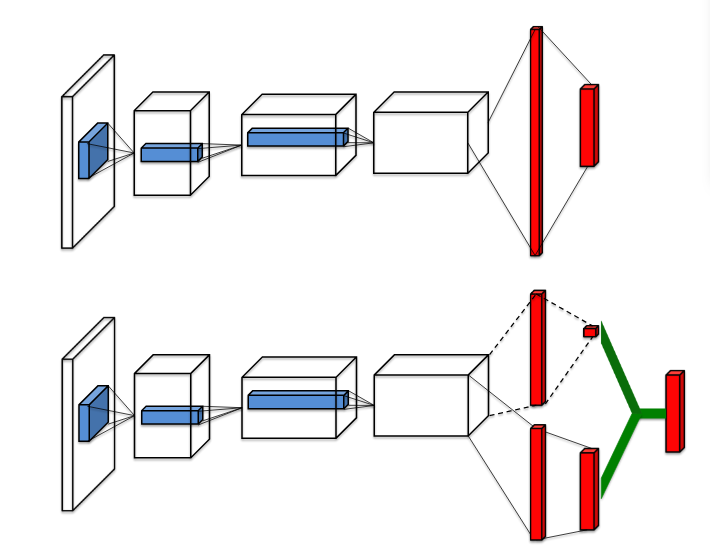
\includegraphics[scale=0.5]{dueling.png}
\caption{Top: Standard Deep Q-network. Bottom: Dueling DQN with two separate streams.\cite{DBLP:journals/corr/WangFL15}}
\label{fig: dueling}
\end{figure}
To exploit this the neural network is split into two streams: 
the action and the state-value stream, as can be seen in figure \ref{fig: dueling}. The benefit of this is, that it is possible to get separate estimations for state-value and action. Hereby the state value $V(s ; \theta_d, \beta)$ is a scalar property while the action-vector $A(s, a ; \theta_d, \alpha)$ has the dimension of the quantity of possible action choices, in our case six. $\theta_d$ are the weights of the network before splitting into two streams, while $\alpha$ and $\beta$ are the weights for the A- and the V- stream respectively.
%TODO How many conv layers, before splitting, how many layers after splitting?
$\theta_d$ are the weights of the network before splitting into two streams, while $\alpha$ and $\beta$ are the weights for the A- and the V- stream respectively.
Now A and V need to be recombined into a Q-value. It is not a good idea though to simply add them:
\begin{equation}
Q(s, a ; \theta, \alpha, \beta)=V(s ; \theta, \beta)+A(s, a ; \theta, \alpha).
\end{equation}
In that case it gets impossible to retrieve V and A from Q uniquely. One could add a constant to A and subtract it from V without changing Q.
It is better to calculate Q by
\begin{equation}
Q(s, a ; \theta, \alpha, \beta)=V(s ; \theta, \beta)+ \left(A(s, a ; \theta, \alpha)-\frac{1}{|\mathcal{A}|} \sum_{a^{\prime}} A\left(s, a^{\prime} ; \theta, \alpha\right)\right),
\end{equation}
where A and V keep their identifiability and the optimization becomes more stable \cite{DBLP:journals/corr/WangFL15}.
\subsection{Noisy Networks}
So far we did use an $\epsilon$-greedy policy for exploration. Another technique which has been found to produce better result for many of the Atari games are Noisy Nets. They add parametric noise to the weights and thus aid exploration without the need to pick random actions as part of a policy (e.g. $\epsilon$-greedy). This is very convenient, because there is no need to tune additional hyper parameters as the reinforcement learning algorithm tunes the weights automatically.
Consider a neural network $y=f_{\theta_n}(x)$. Where $\theta_n$ are the noisy weights. A linear layer of a neural network can be written as: 
\begin{equation}
y = w x+b,
\end{equation}
whereas a noisy linear layer can be written as:
\begin{equation}
y =\left(\mu^{w}+\sigma^{w} \odot \varepsilon^{w}\right) x+\mu^{b}+\sigma^{b} \odot \varepsilon^{b}.
\end{equation}
Here $x$ is the input, $w$, and $\mu^{w}+\sigma^{w} \odot \varepsilon^{w}$ are the weights and $b$ and $\mu^{b}+\sigma^{b} \odot \varepsilon^{b}$ is the bias for linear and noisy linear layer respectively. All of the named parameters are trainable except for $\varepsilon^w$ and $\varepsilon^b$ which are noise random variables. We chose factorized gaussian noise for the distribution of the $\varepsilon$ parameters, as it reduces computation time for random number generation, which is important for single thread-agents such as ours \cite{DBLP:journals/corr/FortunatoAPMOGM17}. Here only one independent noise per input and another independent noise per output is needed, in contrast to independent Gaussian noise, where one independent noise per weight is needed.
We factorized $\varepsilon^w$ to $\varepsilon^w_{i,j}$.
The noise random variables can then be written as:
\begin{equation}
\begin{aligned} \varepsilon_{i, j}^{w} &=f\left(\varepsilon_{i}\right) f\left(\varepsilon_{j}\right) \\ \varepsilon_{j}^{b} &=f\left(\varepsilon_{j}\right) \end{aligned},
\end{equation}
where we used \begin{equation}
f(x)=\operatorname{sgn}(x) \sqrt{|x|}.
\end{equation}
The parameters $\mu_{i,j}$ were initialized as samples from a random uniform distribution $\left[-\frac{1}{\sqrt{p}},+\frac{1}{\sqrt{p}}\right]$ with $p$ being the number of inputs to the noisy linear layer. $\sigma_{i, j}$ were set as $\sigma_{i, j}=\frac{\sigma_{0}}{\sqrt{p}}$. \\
For the Noisy Networks implementation we replaced the Fully Dense layers of the state-value and action streams by Noisy layers. %TODO Loss changes?
\cite{DBLP:journals/corr/FortunatoAPMOGM17}
\subsection{Data augmentation}
As the inputs for our bomberchamp agent are symmetric, we used data augmentation to increase the number of samples for training and to make learning more symmetric.
From each original sample, three augmented samples were created. The augmented samples consist of change of left and right, change of up and down, both combined.
\subsection{Centring of the agent}
To simplify learning for our agent, it was centred on the board, so that it stays at a fixed position while the environment (coins, crates, other agents) move around it. This is very common in the Atari games on which most implementations of DQN agents are tested, including the Rainbow agent without distributional reinforcement learning from which we took most of our initial hyper parameters. Therefore we thought, a more similar setting would be beneficial to our agent. To implement this, the size of the board was increased to four times its original size and the agent placed in the middle of the new board.
\subsection{Self play}
%TODO how was it implemented etc
For training purposes a simple agent implementation that follows the rules of bomberman and plays reasonably well was provided.
To exploit this we wanted to first train our agent by classifying inputs generated with the simple agents. %TODO why didn't this work?
This is why we implemented a self play strategy. This was also useful, as we could then use google colab and train more than one agent at the same time while using the same neural network.



\printbibliography

\end{document}
